\documentclass[11pt]{article}

\usepackage{fancyhdr}
\usepackage{extramarks}
\usepackage{amsmath}
\usepackage{amsthm}
\usepackage{amsfonts}
\usepackage{tikz}
\usepackage[plain]{algorithm}
\usepackage{algpseudocode}
\usepackage{graphicx}
\usepackage{subcaption}
\usepackage{mcode}
\usetikzlibrary{automata,positioning}

%
% Basic Document Settings
%

\topmargin=-0.45in
\evensidemargin=0in
\oddsidemargin=0in
\textwidth=6.5in
\textheight=9.0in
\headsep=0.25in

\linespread{1.1}

\pagestyle{fancy}
\lhead{\hmwkAuthorName}
\chead{\hmwkClass\ (\hmwkClassInstructor\ \hmwkClassTime): \hmwkTitle}
\rhead{\firstxmark}
\lfoot{\lastxmark}
\cfoot{\thepage}

\renewcommand\headrulewidth{0.4pt}
\renewcommand\footrulewidth{0.4pt}

\setlength\parindent{0pt}

%
% Create Problem Sections
%

\newcommand{\enterProblemHeader}[1]{
    \nobreak\extramarks{}{Problem \arabic{#1} continued on next page\ldots}\nobreak{}
    \nobreak\extramarks{Problem \arabic{#1} (continued)}{Problem \arabic{#1} continued on next page\ldots}\nobreak{}
}

\newcommand{\exitProblemHeader}[1]{
    \nobreak\extramarks{Problem \arabic{#1} (continued)}{Problem \arabic{#1} continued on next page\ldots}\nobreak{}
    \stepcounter{#1}
    \nobreak\extramarks{Problem \arabic{#1}}{}\nobreak{}
}

\setcounter{secnumdepth}{0}
\newcounter{partCounter}
\newcounter{homeworkProblemCounter}
\setcounter{homeworkProblemCounter}{1}
\nobreak\extramarks{Problem \arabic{homeworkProblemCounter}}{}\nobreak{}

%
% Homework Problem Environment
%
% This environment takes an optional argument. When given, it will adjust the
% problem counter. This is useful for when the problems given for your
% assignment aren't sequential. See the last 3 problems of this template for an
% example.
%
\newenvironment{homeworkProblem}[1][-1]{
    \ifnum#1>0
        \setcounter{homeworkProblemCounter}{#1}
    \fi
    \section{Problem \arabic{homeworkProblemCounter}}
    \setcounter{partCounter}{1}
    \enterProblemHeader{homeworkProblemCounter}
}{
    \exitProblemHeader{homeworkProblemCounter}
}

%
% Homework Details
%   - Title
%   - Due date
%   - Class
%   - Section/Time
%   - Instructor
%   - Author
%

\newcommand{\hmwkTitle}{Homework\ \#MCMC}
\newcommand{\hmwkDueDate}{12/5/2016}
\newcommand{\hmwkClass}{STAT 5444}
\newcommand{\hmwkClassTime}{}
\newcommand{\hmwkClassInstructor}{Professor Scott Leman}
\newcommand{\hmwkAuthorName}{Kevin Malhotra}

%
% Title Page
%

\title{
    \vspace{2in}
    \textmd{\textbf{\hmwkClass:\ \hmwkTitle}}\\
    \normalsize\vspace{0.1in}\small{Due\ on\ \hmwkDueDate}\\
    \vspace{0.1in}\large{\textit{\hmwkClassInstructor\ \hmwkClassTime}}
    \vspace{3in}
}

\author{\textbf{\hmwkAuthorName}}
\date{}

\renewcommand{\part}[1]{\textbf{\large Part \Alph{partCounter}}\stepcounter{partCounter}\\}

%
% Various Helper Commands
%

% Useful for algorithms
\newcommand{\alg}[1]{\textsc{\bfseries \footnotesize #1}}

% For derivatives
\newcommand{\deriv}[1]{\frac{\mathrm{d}}{\mathrm{d}x} (#1)}

% For partial derivatives
\newcommand{\pderiv}[2]{\frac{\partial}{\partial #1} (#2)}

% Integral dx
\newcommand{\dx}{\mathrm{d}x}

% Alias for the Solution section header
\newcommand{\solution}{\textbf{\large Solution}}

% Probability commands: Expectation, Variance, Covariance, Bias
\newcommand{\E}{\mathrm{E}}
\newcommand{\Var}{\mathrm{Var}}
\newcommand{\Cov}{\mathrm{Cov}}
\newcommand{\Bias}{\mathrm{Bias}}

\begin{document}

\maketitle

\pagebreak

\begin{homeworkProblem}
\begin{align*}
&Assume: \pi(x)g(x'|x) \leq \pi(x')g(x|x') \\
&x\rightarrow x' \\
&\alpha_{MH}(x'|x) = Min\bigg(1, \frac{\pi(x')}{\pi(x)}\frac{g(x|x')}{g(x'|x)}\bigg) = 1 \\
&p(x'|x) = g(x'|x)\alpha_{MH}(x'|x) = g(x'|x) \\
&x'\rightarrow x \\
&\alpha_{MH}(x'|x) = Min\bigg(1, \frac{\pi(x)}{\pi(x')}\frac{g(x'|x)}{g(x|x')}\bigg) =  
	\frac{\pi(x)}{\pi(x')}\frac{g(x'|x)}{g(x|x')} \\
&p(x|x') = g(x|x')\alpha_{MH}(x|x') = g(x|x') \frac{\pi(x)}{\pi(x')}\frac{g(x'|x)}{g(x|x')} \\
&p(x|x')p(x') = p(x'|x)p(x) \\
&g(x|x') \frac{\pi(x)}{\pi(x')}\frac{g(x'|x)}{g(x|x')} p(x') = g(x'|x)p(x) \\
&\frac{\pi(x)}{\pi(x')}\frac{g(x'|x)}{g(x|x')} = \frac{p(x)}{p(x')} \\
\end{align*}
This solution describes that both steps of the transitions end up being symmetric which  concludes that the \(\pi(x)\) is the stationary distribution for this Markov chain.
\end{homeworkProblem}
\begin{homeworkProblem}
\begin{align*}
\alpha_{MH} &= \bigg(1, \frac{\pi(\theta^*)}
	{\pi(\theta)}\frac{g(\theta|\theta^*)}{g(\theta^*|\theta)}\bigg) \\
\alpha_{MH} &= Min\bigg(1, \frac{\pi(\mu^* \phi^*)}{\pi(\mu\phi)}
	\frac{g(\mu, \phi| \mu^* \phi^*)}{g(\mu^* \phi^*|\mu, \phi)}\bigg) \\
\alpha_{MH} &= Min\bigg(1, \frac{\pi(\mu^* \phi^*)}{\pi(\mu\phi)}
	\frac{g(\mu|\mu^*)g(\phi|\phi^*)}{g(\mu^*|\mu)g(\phi^*|\phi)}\bigg) \\
\alpha_{MH} &= Min\bigg(1, 
	\frac{\phi^{*(\frac{n}{2}-1)}exp(-\frac{\phi^*}{2}\sum_{i=1}^N (x_i-\mu^*)^2)}
	{\phi^{(\frac{n}{2}-1)}exp(-\frac{\phi}{2}\sum_{i=1}^N (x_i-\mu)^2)}
	\frac{exp(\frac{-1}{2}(\mu-\mu^*)^2)}{exp(\frac{-1}{2}\mu^*-\mu)^2)}
	\frac{ g(\phi|\phi^*)}{g(\phi^*|\phi)}\bigg) \\
\alpha_{MH} &= Min\bigg(1, 
	\frac{\phi^{*(\frac{n}{2}-1)}exp(-\frac{\phi^*}{2}\sum_{i=1}^N (x_i-\mu^*)^2)}
	{\phi^{(\frac{n}{2}-1)}exp(-\frac{\phi}{2}\sum_{i=1}^N (x_i-\mu)^2)}
	\frac{exp(\frac{-1}{2}(\phi-\phi^*)^2)}{\Phi(\phi)}\frac{\Phi(\phi^*)}
	{exp(\frac{-1}{2}(\phi-\phi^*)^2)}\bigg) \\
\alpha_{MH} &= Min\bigg(1, 
	\frac{\phi^{*(\frac{n}{2}-1)}exp(-\frac{\phi^*}{2}\sum_{i=1}^N (x_i-\mu^*)^2)}
	{\phi^{(\frac{n}{2}-1)}exp(-\frac{\phi}{2}\sum_{i=1}^N (x_i-\mu)^2)}
	\frac{\Phi(\phi^*)}{\Phi(\phi)}\bigg) \\
\end{align*}
\begin{figure*}[t!]
    \centering
    \begin{subfigure}[t]{0.3\textwidth}
        \centering
		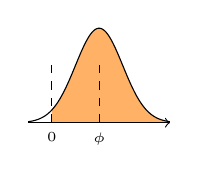
\begin{tikzpicture}[scale=0.3]
		\def\normalt{\x,{4*1/exp(((\x-3)^2)/2)}}
		\def\y{1}
		\def\fy{4*1/exp(((\y-3)^2)/2)}
		%Fill
		\fill [fill=orange!60](1,0)--plot[domain=1:6](\normalt)--(4.0,0)-- cycle;
		%Descriptions
		\draw[dashed] (1.0,0) node[below] {\tiny{0}} --+ (0,2.75);
		\draw[dashed] (3.0,0) node[below] {\tiny{\(\phi\)}} --+ (0,2.75);
		%Plot
		\draw[color=black,domain=0:6] plot[samples=1000] (\normalt) node[right] {};
		%Axes
		\draw[->] (0,0) -- (6,0) node[right] {$$};
		\end{tikzpicture}
        \caption{Figure 1}
    \end{subfigure}%
    \begin{subfigure}[t]{0.3\textwidth}
        \centering
		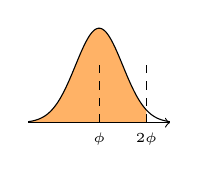
\begin{tikzpicture}[scale=0.3]
		\def\normalt{\x,{4*1/exp(((\x-3)^2)/2)}}
		\def\y{1}
		\def\fy{4*1/exp(((\y-3)^2)/2)}
		%Fill
		\fill [fill=orange!60](2,0)--plot[domain=0:5](\normalt)--(5.0,0)-- cycle;
		%Descriptions
		\draw[dashed] (3.0,0) node[below] {\tiny{\(\phi\)}} --+ (0,2.75);
		\draw[dashed] (5.0,0) node[below] {\tiny{\(2\phi\)}} --+ (0,2.75);
		%Plot
		\draw[color=black,domain=0:6] plot[samples=1000] (\normalt) node[right] {};
		%Axes
		\draw[->] (0,0) -- (6,0) node[right] {$$};
		\end{tikzpicture}
        \caption{Figure 2}
    \end{subfigure}%
    \begin{subfigure}[t]{0.3\textwidth}
		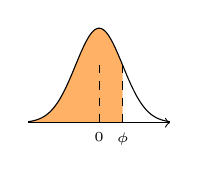
\begin{tikzpicture}[scale=0.3]
		\def\normalt{\x,{4*1/exp(((\x-3)^2)/2)}}
		\def\y{1}
		\def\fy{4*1/exp(((\y-3)^2)/2)}
		%Fill
		\fill [fill=orange!60](2,0)--plot[domain=0:4](\normalt)--(4.0,0)-- cycle;
		%Descriptions
		\draw[dashed] (3.0,0) node[below] {\tiny{0}} --+ (0,2.75);
		\draw[dashed] (4.0,0) node[below] {\tiny{\(\phi\)}} --+ (0,2.75);
		%Plot
		\draw[color=black,domain=0:6] plot[samples=1000] (\normalt) node[right] {};
		%Axes
		\draw[->] (0,0) -- (6,0) node[right] {$$};
		\end{tikzpicture} 
        \caption{Figure 3}
    \end{subfigure}%
    \caption{CDF Plots}
\end{figure*} \\ \\ \\
\-\(\Phi(\phi) \) is the cdf up to some phi. The reason we need to apply this normalization is that since we are in a truncated space these normalizations will not cancel out and will affect the final target distribution. The CDFs functions in matlab require the CDF calculations to be transformed in a specific manner. The first plot above is the target area we want to cover which is equivalent to the second plot because they cover the same space since we cover half of the area + an area spanning \(\phi\). The second and third plots are equivalent since normal distributions are shift invariant so we can just scale the center. Thus the final distribution follows a standard normal cdf which is \( \int_{-\infty}^\phi e^{\frac{-1}{2}x} dx \)
\begin{align*}
\sigma_{\phi}^2 &= 1 \\
\sigma_{\mu}^2 &= 1000 \\
\mu_0 &= 0 \\
\phi_0 &= 5 \\
For&\rightarrow t=2:T \\
1.& \mu*- N(\mu_{t-1}, \sigma_{\mu}^2) \\
2.& \phi* - N(\phi_{t-1}, \sigma_{\phi}^2) \\
3.& \alpha_{MH} = Min\bigg(1, 
	\frac{\phi^{*(\frac{n}{2}-1)}exp(-\frac{\phi^*}{2}\sum_{i=1}^N (x_i-\mu^*)^2)}
	{\phi_{t-1}^{(\frac{n}{2}-1)}exp(-\frac{\phi_{t-1}}{2}\sum_{i=1}^N (x_i-\mu_{t-1})^2)}
	\frac{\frac{\Phi(\phi^*)}{\sigma_{\phi}^2}}{\frac{\Phi(\phi_{t-1})}{\sigma_{\phi}^2}}\bigg) \\
4.& \pi(\mu, \phi) = \phi^{*(\frac{n}{2}-1)}exp(-\frac{\phi}{2}\sum_{i=1}^N (x_i-\mu)^2) \Phi(\phi) \\
5.&if(log(unif(0, 1) \leq \big[log(\pi(\mu^*, \phi^*)) - log(\phi(\mu_{t-1}, \phi_{t-1}))\big]) 
	Lemma: (\frac{\pi(\mu^*, \phi^*)}{\pi(\mu_{t-1}, \phi_{t-1})} \leq unif(0, 1) < 1) \\
	&\mu_t, \phi_t = \mu^*, \phi^* \\
	el&se \\
	&\mu_t, \phi_t = \mu_{t-1}, \phi_{t-1} \\
en&d\\
end&
\end{align*}
\includegraphics[scale=0.3]{Part2Attempt1.png} \\
Burn-in Time = 200 Iterations \\
\lstinputlisting{MH.m}
\end{homeworkProblem}
\pagebreak
\begin{homeworkProblem}
\lstinputlisting{GibbsPart3.m}
K = 2, K = 5 \\	
\includegraphics[scale=0.4]{k2.png} \includegraphics[scale=0.20]{k5p2.png}\\ 
K = 20, K = 50 \\
\includegraphics[scale=0.20]{k20.png} \includegraphics[scale=0.20]{k50Attempt3.png}\\ 
\end{homeworkProblem}
\pagebreak
\begin{homeworkProblem}
\textbf{Introduction:} \\
\-\hspace{10mm} Gaussian Mixture Models provide the ability to take an arbitrary set of data and generate a target distribution through Monte Carlo Markov Processes. This process works when we know how many modes or components need to be modeled to approach the target distribution. For a given component there is a mean, standard deviation, and weighting for the Gaussian. Each weighting is defined as the probability or a given data point to be in a specific cluster. Therefore, every single data point has a probability to be in each component. Given these constraints the appropriate assignments to data points must be made to generate the Gaussian Mixture Model to fit the dataset. For the problem, simulations must be performed with different number of components, a random data set that will be generated, and hyper parameters tuning to understand Gaussian Mixture Models.\\
\textbf{Procedure:} \\
\-\hspace{10mm} The following problem was approached by using Gibbs Sampling Procedure, a Monte Carlo Markov Process, to converge towards the solution. The first problem to solve is how to generate the data. Given the number of data points that need to be generated a Multinomial distribution is used with equal weights to determine how many samples are coming from each Gaussian distribution. The data is randomized and stored in an entire vector. Initialization of all the parameters for each component is done by setting each components parameters skewed away from the mean by some arbitrary amount. This tuning is changed throughout the testing and it affects the convergence of the algorithm. \\
\-\hspace{10mm} The algorithm is split up into two sections. The first section focusing on keeping the Gaussian component parameters the same and updating the data point assignments. The second section focusing on keeping the data point assignments the same and updating the Gaussian component parameters. The first step is done by acquiring the conditional probability for a data point to belong in a cluster. The equation formulates to be \( P(C_i = j | x_i, \theta_1, ... \theta_J) = \frac{P(x_i|\theta_j, C_i = j)P(C_i = j)}{\sum_{i=1}^JP(x_i|\theta_j, C_i = j)P(C_i = j)}\) where \(C_i\) refers to the current component and \(\theta_j\) refers to the component's parameters. This is sampled for every possible component and data point. This will generate a NxJ matrix of probabilities. In the algorithm, everything is computed in log form for numerical stability and vectorized for speed. For a given data point and it's J probabilities for the J respective components a cluster assignment must be made. The cluster assignment is done by a Multinomial(Categorical since 1 sample is needed) which generates an assignment based on the probabilities. The assignments are updated for every data point and the second step must be performed. \\
\-\hspace{10mm} The second step requires using the posterior distributions for the Gaussian parameters. The Jeffrey's Priors are used for \(\mu\propto1\) and \(\phi\propto\frac{1}{\phi}\). The likelihood function chosen are the standard Normal Distribution for \(\mu\) and Gamma Distribution for \(\phi\). These generate the posterior distributions \( \mu_j - N(\bar{x}^j, \frac{1}{\phi_j N_j}) \) and \( \phi_j - Gamma(\frac{N_j}{2}, \frac{\sum_{i=1}^N (x_i^j - \mu_j)^2}{2})\). The j subscripts represent the subset of the entire datasets component assignments. As a result of the first step, the Gaussian components are updated by using the component assignments to sample from the posterior distribution for a new Gaussian components. These updated parameters will be used in the next step to update the cluster assignments. This process will lead to the convergence and oscillations around the ground truth. \\
\textbf{Simulations Results:} \\
\-\hspace{10mm} After performing all the simulations across J = 2, 5, 20, 50. I have come across a few results during simulation. When two means of each component are close together they begin to oscillate around the two means, there is a certain threshold to this. I was able to get the true means within 2 units of each other when the components would begin to oscillate around the two means. One of the other issues facing convergence was having the correct number of points for all the components. If there were not enough points for each component then the model would also fail to converge and may miss an component completely. As, I kept increasing the component values, these two major cases had to be in mind when performing initialization. Without the appropriate hyper parameter tuning for each component the model would not converge; therefore, smart initialization is required to tweak the sampler to generate the correct distribution. \\
\includegraphics[scale=0.25]{k5p2.png} \includegraphics[scale=0.25]{k50Attempt3.png}\\ 
The first image contains the issue of oscillating between two different means. The second image is the 50 component model converging towards the solution. As the variance of each component increased so did the oscillations of that variable when it was converging towards the solution. \\
\textbf{Numerical Stability:} \\
Numerical Stability was faced throughout the implementation of the entire implementation. The probability equation was converted to log form. The following equation must be put into log form and it required a few derivations to get it completely correct \( P(C_i = j | x_i, \theta_1, ... \theta_J) = \frac{P(x_i|\theta_j, C_i = j)P(C_i = j)}{\sum_{i=1}^JP(x_i|\theta_j, C_i = j)P(C_i = j)}\). The final derivation for the denominator is \( log(\sum_{j=1}^J e^{log(\pi_{max}(x)) - log (\pi_j(x))}) \). This final form was used to to retain numerical stability. \\
\textbf{Conclusions:} \\
The sampler is extremely good at performing and it is relatively fast. As I increased the components the data points also had to be increased to allow for a good mass for each component. This caused an increased complexity and it remained near linear time in terms of performance. The sampler converges in relatively small iterations but it is run longer to see the oscillation changes. The biggest issues faced were the numerical stability problems and the figuring out that the number of points was a factor of convergence. Matlab also has different gamma functions which made it difficult to find numerical errors. Overall, the sampler is relatively fast and vectorized and it is clear and works without numerical problems.
\end{homeworkProblem}
\end{document}
